\documentclass{beamer}
\usetheme{Frankfurt}
\usepackage{fontspec}
\usepackage{graphicx}
\usepackage{tikz}
\usepackage[english,russian]{babel}
\usepackage{xltxtra}
\usepackage{xunicode}
\setbeamertemplate{navigation symbols}{}
\setbeamertemplate{footline}{}
\defaultfontfeatures{Scale=MatchLowercase,Mapping=tex-text}
\begin{document}
\newcommand{\fn}{\fontspec{Arial}}
\fn
\setbeamerfont{listfn}{size=\Large}
\setbeamerfont{resetfn}{size=\normalsize}
\title{Система обліку платних курсів. Модуль обліку платних курсів}
\author{Студент --- Горбешко Б. М.\\Керівник --- Оніщенко Т. В.}
\date{}
\frame{\titlepage}
\begin{frame}{\fn Причина і мета розробки}
Причиною розробки автоматизованої системи обліку платних курсів є відсутність такої системи на кафедрі Системного програмного забезпечення.

Метою створення системи є розробка комп'ютерної системи обліку платних курсів для зменшення часу роботи працівників кафедри зі слухачами шляхом автоматизації набору слухачів на курси, реєстрацій сплат та формування звітності, а також для надання майбутнім слухачам можливості ознайомитися з наявними курсами та залишити заявку на реєстрацію за допомогою зовнішніх програмних сервісів.
\end{frame}
\begin{frame}{\fn Діаграма концептуальних класів}
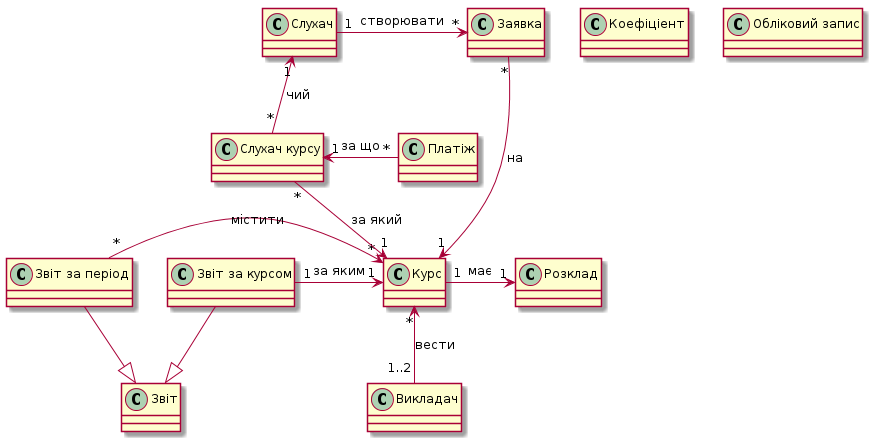
\includegraphics[width=10cm]{pp_pw3_conc.png}
\end{frame}
\begin{frame}{\fn Вимоги}
\begin{itemize}
\item Робота з слухачами, курсами, викладачами, розкладом, сплатами за курси
\item Відображення та редагування даних у таблицях
\item Формування придатних до друку звітів
\item Web-інтерфейс
\item Вкладені таблиці для сутностей M--M
\end{itemize}
\end{frame}
\begin{frame}{\fn Аналогічні системи}
\begin{itemize}
\item 1C: Бухгалтерія
\item Парус
\item 1C-Бітрікс: Внутрішній портал навчального закладу
\item Moodle
\item Веб-застосунок MS Access + SharePoint
\end{itemize}
\end{frame}
\begin{frame}{\fn Діаграма прецедентів}
\begin{center}
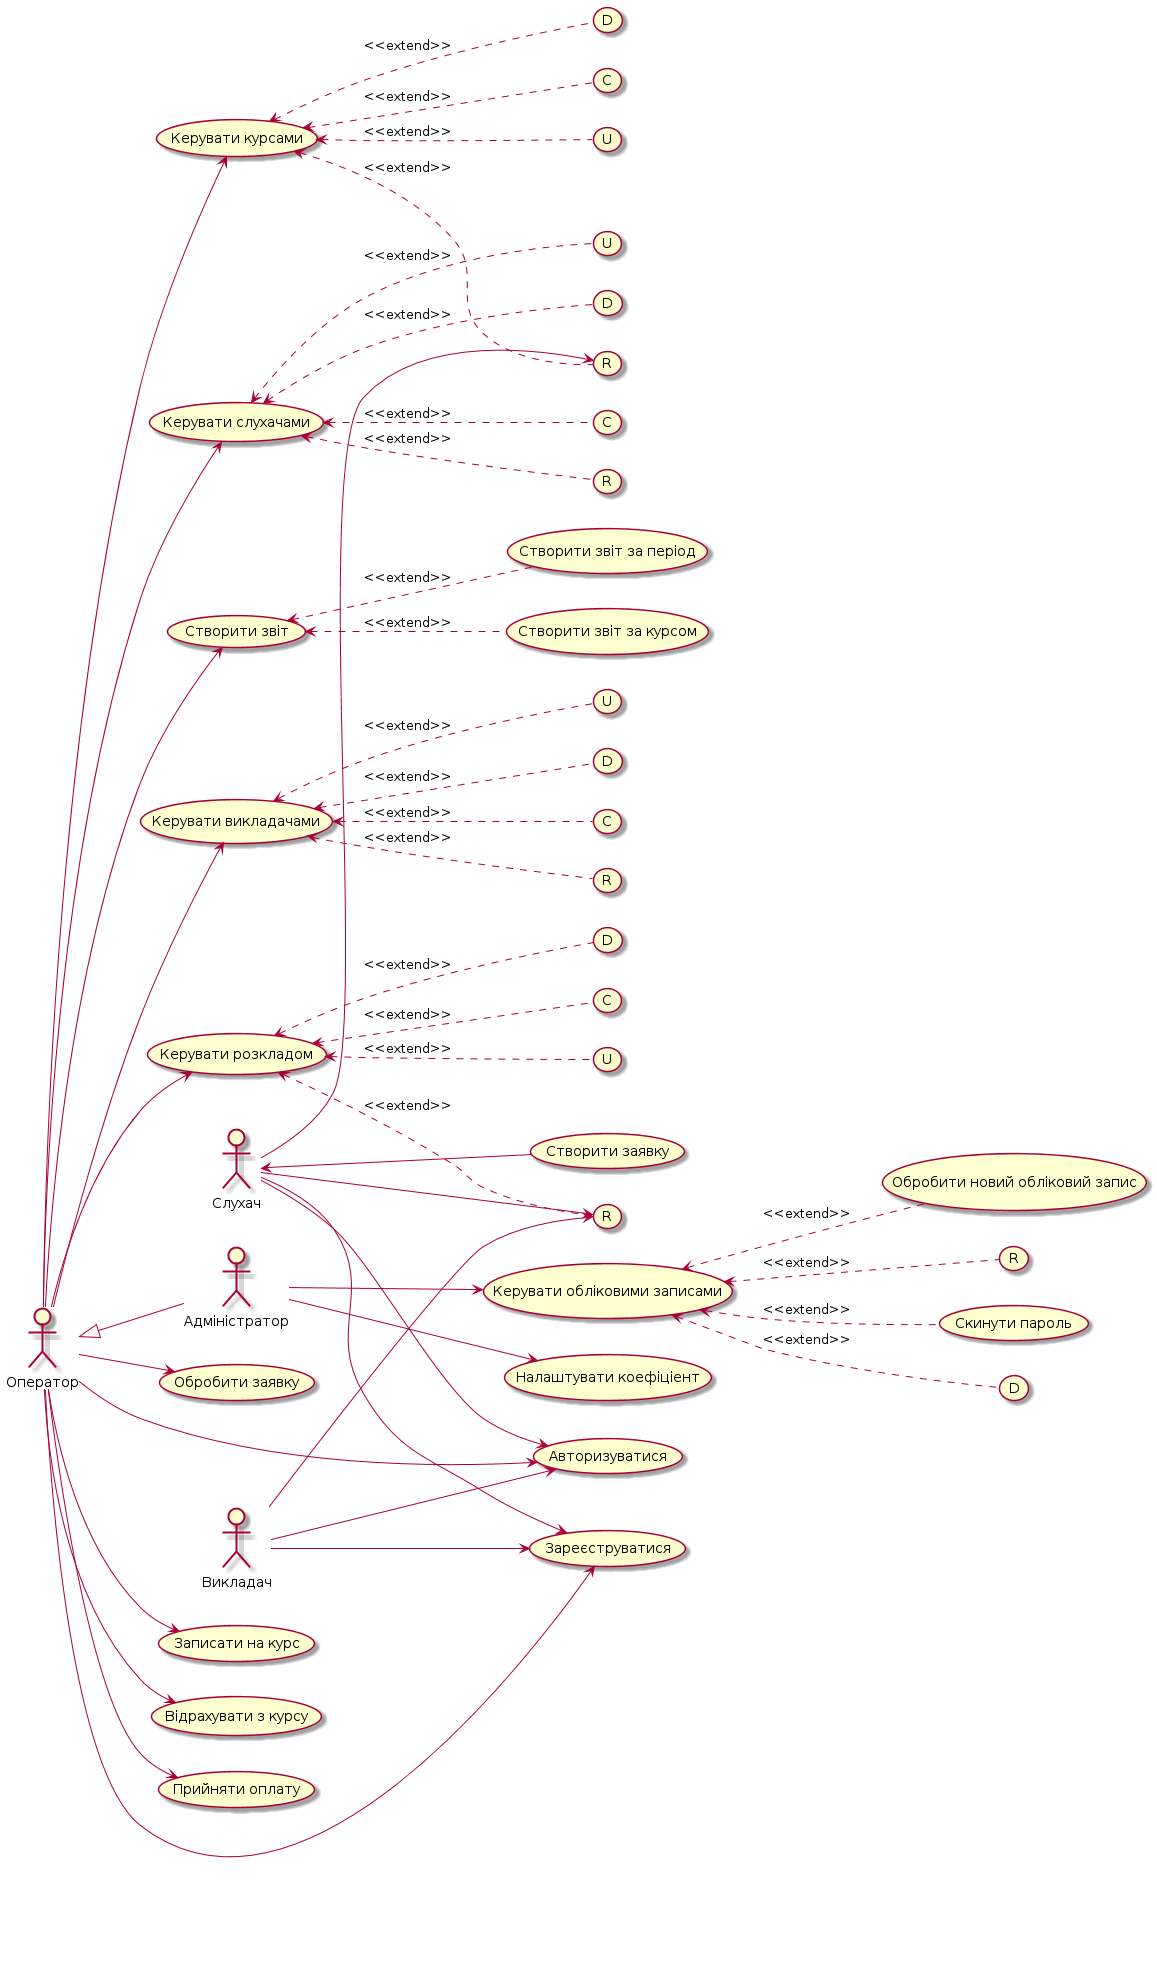
\includegraphics[width=5cm]{pp_pw1_uc.png}
\end{center}
\end{frame}
\begin{frame}{\fn Діаграма програмних класів}
\begin{center}
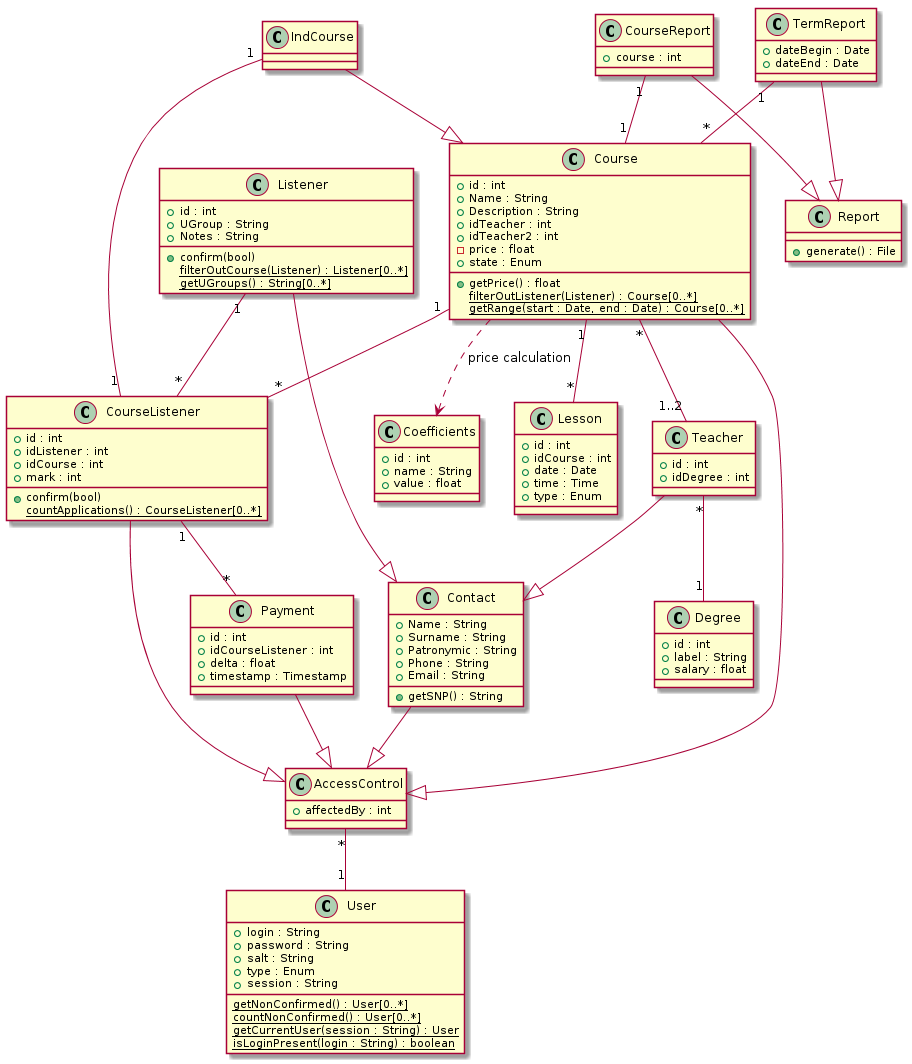
\includegraphics[width=7cm]{pp_pw3_clas.png}
\end{center}
\end{frame}
\begin{frame}{\fn Головне меню системи}

\includegraphics[width=11cm]{scrns/menu.png}
\end{frame}
\begin{frame}{\fn Приклад таблиці}
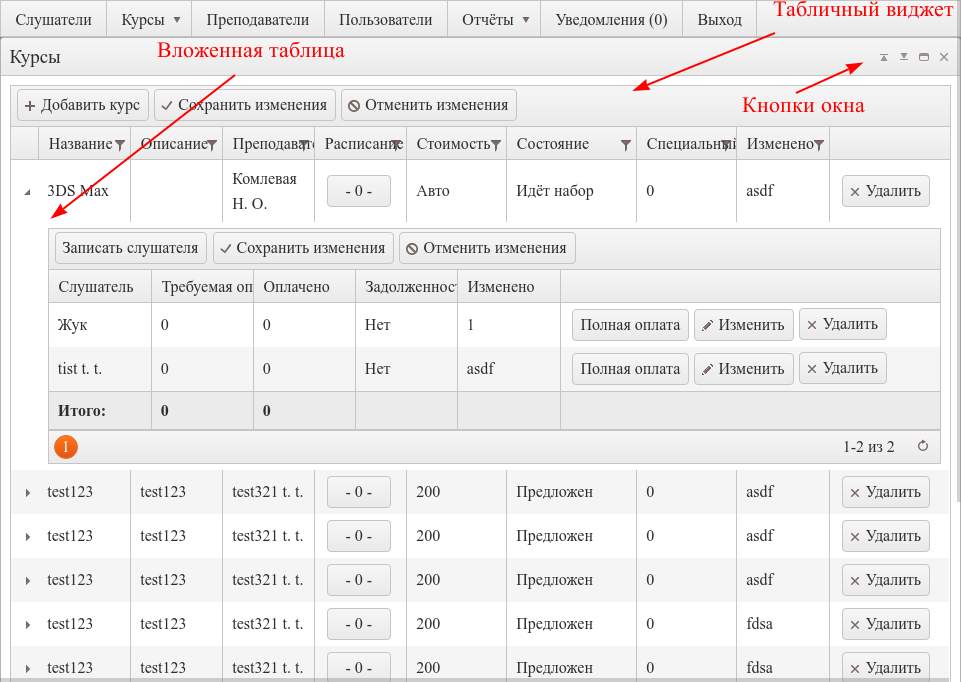
\includegraphics[width=10cm]{scrns/scrn3.png}
\end{frame}
\begin{frame}{\fn Сповіщення}
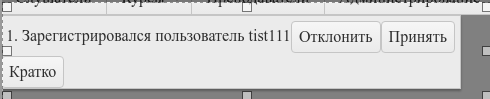
\includegraphics[width=10cm]{scrns/notifications.png}
\end{frame}
\begin{frame}{\fn Звіт}
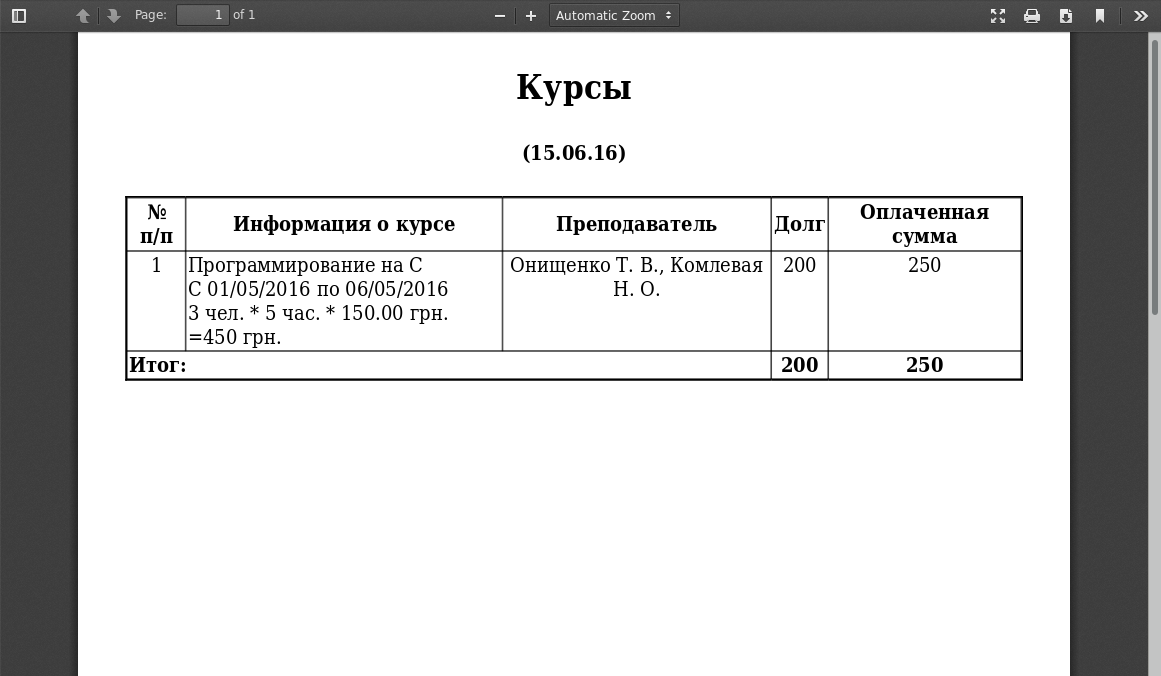
\includegraphics[width=10cm]{scrns/report.png}
\end{frame}
\begin{frame}{}
\begin{center}
{\fontsize{48pt}{48pt}\selectfont Дякую за увагу!}
\end{center}
\end{frame}
\end{document}
